% sudo apt update && sudo apt install -y texlive-full
% 使用 XeLaTeX 编译: xelatex thesis.min.tex
% CCF 中国计算机学会 A 类会议论文格式
% Swift: 启发式多信号融合自适应网络拥塞控制算法

\documentclass[10pt,twocolumn]{article}

% 中文支持
\usepackage[UTF8]{ctex}
\usepackage{fontspec}

% 数学公式
\usepackage{amsmath}
\usepackage{amssymb}

% 图表
\usepackage{graphicx}
\usepackage{float}
\usepackage{booktabs}
\usepackage{multirow}
\usepackage{array}

% 算法
\usepackage{algorithm}
\usepackage{algorithmic}

% 引用和链接
\usepackage{cite}
\usepackage{hyperref}
\usepackage{url}

% 颜色
\usepackage{xcolor}

% 页面设置
\usepackage{geometry}
\geometry{a4paper,left=1.9cm,right=1.9cm,top=2.2cm,bottom=2.2cm,columnsep=0.55cm}

% 行距
\usepackage{setspace}
\setstretch{1.08}

% 标题间距
\usepackage{titlesec}
\titlespacing*{\section}{0pt}{10pt}{5pt}
\titlespacing*{\subsection}{0pt}{7pt}{3pt}
\titlespacing*{\subsubsection}{0pt}{5pt}{2pt}
\titleformat{\section}{\normalfont\large\bfseries}{\thesection}{0.5em}{}
\titleformat{\subsection}{\normalfont\normalsize\bfseries}{\thesubsection}{0.5em}{}
\titleformat{\subsubsection}{\normalfont\small\bfseries}{\thesubsubsection}{0.5em}{}

% 紧凑列表
\usepackage{enumitem}
\setlist{nosep,leftmargin=1.2em}

% caption
\usepackage{caption}
\captionsetup{font=small,labelfont=bf,skip=4pt}

% 浮动体间距
\setlength{\textfloatsep}{8pt plus 2pt minus 2pt}
\setlength{\floatsep}{6pt plus 2pt minus 2pt}
\setlength{\intextsep}{6pt plus 2pt minus 2pt}
\setlength{\abovecaptionskip}{4pt}
\setlength{\belowcaptionskip}{2pt}

% 段落间距
\setlength{\parskip}{1.5pt plus 0.5pt minus 0.5pt}

% 算法环境字体
\usepackage{etoolbox}
\AtBeginEnvironment{algorithmic}{\small}

%% 英文字体默认使用 Times New Roman
\RequirePackage{xltxtra} % \XeTeX Logo
\setmainfont{Times New Roman}   % 衬线字体
\setsansfont{Arial}             % 无衬线字体
\setmonofont{Courier New}       % 等宽字体，一般是打印字体
%% 中文字体默认使用宋体
%\setCJKmainfont{songti}
\IfFontExistsTF{STXingkai}{
  \setCJKfamilyfont{hwxk}{STXingkai} % Windows
}{
  \setCJKfamilyfont{hwxk}{Sarasa Gothic SC} % Other
}
\newcommand{\stxk}{\CJKfamily{hwxk}}
\IfFontExistsTF{SimSun}{
  \setCJKfamilyfont{zhsong}[AutoFakeBold = {2.17}]{SimSun} % Windows
}{
  \setCJKfamilyfont{zhsong}[AutoFakeBold = {2.17}]{Sarasa Gothic SC} % Other
}
%\renewcommand{\songti}{\CJKfamily{zhsong}}

\begin{document}

%========================================
% 标题
%========================================

\title{\Large\textbf{Swift: 启发式多信号融合自适应网络拥塞控制算法}}

\author{
\normalsize 杭天铖 \\
\small 南京邮电大学 \\
\small 1224045520@njupt.edu.cn
}

\date{}

\maketitle

%========================================
% 摘要
%========================================

\begin{abstract}
\small
端到端网络传输的服务对象正在从固定终端和近端高质量链路，扩展到跨地域远距离传输、蜂窝/无线/卫星等多接入路径，以及手机、笔记本、台式机和边缘设备等异构终端并存的复杂场景。传统基于丢包的算法存在拥塞信号滞后与缓冲区膨胀问题，基于延迟的算法面临RTT测量噪声与共存公平性不足等挑战；当端点、链路、RTT和业务条件同时变化时，固定参数、单一信号驱动的拥塞控制更难兼顾吞吐、时延与稳定性。本文提出Swift——一种面向上述广泛端到端传输场景的启发式多信号融合自适应拥塞控制方法，其核心创新收敛为三点：（1）\textbf{多信号拥塞状态感知}，将ECN状态、拥塞避免状态机状态、拥塞事件语义、RTT与最小RTT、在途字节等协议栈内部信息组织为11维有效观测子空间（嵌入含4项路由元数据的15元素传输容器），并以两级优先级判定区分超时、ECN触发的窗口收缩与普通丢包；（2）\textbf{ns3-gym集成的事件驱动启发式融合控制}，在\texttt{GetSsThresh}与\texttt{IncreaseWindow}回调处经同步请求--应答交换动作$[new\_ssThresh,new\_cWnd]$，由最小RTT感知的RTT膨胀比、反馈值相对慢速基线的偏移和连续增长趋势调节每流$\alpha\in[0.85,1.30]$，并以有界步长逼近由滑动时间窗投递速率最大值滤波得到的$\alpha\times BDP$目标窗口；（3）\textbf{面向不确定拥塞信号的稳定性与安全机制}，包括差异化窗口保留因子（丢包0.70、ECN 0.75、超时0.50）、至多3次连续缩减、降窗后4个ACK事件冻结、基于$\min(cwnd,BDP)$的慢启动阈值更新、窗口钳位以及CA\_LOSS下的陈旧动作失效。该控制器为确定性白盒Python启发式，不是端到端训练的强化学习策略。

在ns-3.40离散事件仿真平台上，本文以哑铃拓扑和3条并发长流评估Swift。36个命名场景是对近端高速、共享汇聚、无线/蜂窝接入、城域/跨域广域网与LEO/GEO卫星链路参数的剖面化模拟，并非对手机、笔记本或台式机硬件的直接建模；瓶颈为10 Mbps$\sim$100 Gbps，基线RTT为4 $\mu$s$\sim$640 ms。纯TCP与UDP突发两种设置共形成288条协议记录；突发流的平均负载为瓶颈速率32\%，On期峰值为64\%，占空比为50\%。按ns-3 FlowMonitor的前向TCP数据流统计，纯TCP设置下Swift在所考察场景中整体呈现吞吐领先，相对逐场景最强基线的增益为2.1\%$\sim$5.8\%（中位数与均值均约4.1\%）；Swift严格时延最低的场景为7个，在21/36个场景中与最低时延相差不超过2\%，Jain指数在32/36个场景中距最优值不超过0.002，而严格丢包率最低仅见于8个场景。UDP突发下，相对最强基线的吞吐增益为2.2\%$\sim$5.9\%（均值3.7\%），吞吐保持率均值为68.6\%，与基线可比。代表性结果包括长途WAN、LEO卫星、LTE弱覆盖和500 Mbps近端链路等参数剖面；混合结果则包括传统WiFi、5G边缘和GEO卫星等时延不占优的场景。公平性与丢包整体接近基线，而非统一最优。每个配置仅运行一个随机运行号，本文不作置信区间或统计显著性声明。

\vspace{0.3em}
\noindent\textbf{关键词：}拥塞控制；启发式自适应；多信号融合；显式拥塞通知；自适应参数调优；远距离传输；异构终端
\end{abstract}

%========================================
% 1. 引言
%========================================

\section{引言}

随着云计算、大数据、人工智能、移动互联网和物联网技术的蓬勃发展，端到端网络传输的服务对象正在从固定主机扩展到手机、笔记本、台式机、边缘节点和传感设备等异构终端，传输路径也从近端局域链路延伸到跨城、跨域、蜂窝接入、无线局域网和卫星通信等远距离复杂网络。TCP作为互联网传输层的核心协议，其拥塞控制机制的性能直接影响网络资源利用效率、应用响应延迟和用户体验。

在这类端到端传输场景中，网络路径和终端侧条件呈现出更强的异构性。一方面，城域/广域网、蜂窝网络、WiFi与卫星链路具有不同的RTT量级、丢包背景、可用带宽和链路抖动；另一方面，手机、笔记本、台式机和边缘设备等端点在处理能力、接入方式、移动性和业务负载上存在差异。同一拥塞控制策略需要适应从短RTT近端高速链路到长RTT远距离链路的变化，并应对突发跨流量、无线误码和终端负载波动。上述复杂性使传统依赖固定参数或单一拥塞信号的算法难以同时兼顾吞吐、时延和稳定性。

传统基于丢包的拥塞控制算法（如NewReno\cite{newreno}、CUBIC\cite{cubic}）将丢包作为拥塞信号，但丢包通常是较滞后的拥塞指示，可能伴随缓冲区占用和排队时延上升，形成Bufferbloat问题\cite{bufferbloat}。Vegas\cite{vegas}等基于时延的算法尝试通过RTT变化提前感知拥塞，BBR\cite{bbr}则估计瓶颈带宽与传播RTT；这类测量可能受路径抖动、终端调度和接入条件变化影响，与其他算法共存时也需专门评估公平性\cite{bbrfairness}。

ECN机制\cite{rfc3168}允许网络设备在发生拥塞且报文支持ECN时进行标记，而不必仅依赖丢包传递信号。DCTCP\cite{dctcp}利用ECN标记比例进行细粒度调整。不同算法对ECN、RTT、丢包和协议栈状态的组合方式不同，如何在多样端点与路径条件下联合解释这些信号仍值得研究。

近年来，强化学习在网络拥塞控制中的应用受到关注\cite{rlcc}。Aurora\cite{aurora}采用PPO算法训练深度神经网络策略，Orca\cite{orca}使用强化学习动态调整AIMD参数；SIGCOMM 2023的Sage\cite{sage2023}进一步将经典启发式控制知识融入学习过程，以改善策略训练和真实互联网环境中的表现。然而，这类学习型方案通常需要训练与模型推理设施，其多目标权衡和训练分布外行为需要专门验证。本文选择另一设计点：以协议栈内部信号驱动的\emph{白盒启发式规则}作为决策主体，仅在参数层进行轻量反馈调整，使控制路径可逐分支检查且不依赖训练样本。

与单一网络域相比，跨地域和多接入传输的拥塞信号更难解释。丢包可能来自真实队列溢出，也可能来自无线误码或链路切换；RTT升高既可能表示排队，也可能来自路径变化、终端调度延迟或接入链路抖动；突发UDP/RPC/视频/备份流量还会造成短时间带宽挤占。近期发表于IEEE/ACM ToN的MPLibra\cite{mplibra2024}也表明，在异构多路径环境中结合经典控制与学习决策是一条值得探索的路线。因此，Swift的设计目标不是某一类专用网络，而是服务远距离传输、手机/笔记本/台式机等异构端点以及多样接入与路径条件的通用端到端传输。相应地，本文将微秒级RTT近端高速链路、无线局域网、蜂窝接入、城域/跨域广域网与卫星链路组织为覆盖不同RTT、带宽和跨流量条件的评估集合；这些场景模拟链路与路径参数，并不等同于对具体终端硬件的验证。

针对上述挑战，本文提出Swift算法——一种启发式多信号融合自适应网络拥塞控制方法。ns-3侧在\texttt{GetSsThresh}和\texttt{IncreaseWindow}回调处通过ns3-gym/OpenGym\cite{opengym}同步请求--应答路径交换15元素观测容器与二元素动作；\texttt{PktsAcked}、\texttt{CongestionStateSet}和\texttt{CwndEvent}负责更新RTT、拥塞状态、事件及陈旧动作状态。协议栈外的Python控制器据此执行确定性规则，而非端到端训练策略。本文的核心创新收敛为如下三点：

\textbf{（1）面向远距离与异构端点的多信号拥塞状态感知}：将ECN状态、拥塞避免状态机状态、拥塞事件语义、RTT与最小RTT、在途字节等协议栈内部信息组织为11维有效观测子空间，并以两级优先级判定区分超时、ECN触发的窗口收缩与普通丢包，为多样接入与路径条件提供联合判定依据。

\textbf{（2）ns3-gym集成的事件驱动启发式融合控制}：由最小RTT感知的RTT膨胀比、性能反馈值相对其慢速基线的偏移量以及连续增长趋势共同调节每流乘性增加因子$\alpha \in [0.85, 1.30]$，并以有界步长逼近$\alpha \times BDP$目标窗口；BDP由滑动时间窗口累计确认字节计算的投递速率及40样本最大值滤波给出，并结合最小RTT感知的HyStart风格慢启动退出和管道利用率感知增量。

\textbf{（3）面向不确定拥塞信号的稳定性与安全机制}：依据信号类别施加差异化窗口保留因子（丢包0.70、ECN 0.75、超时0.50），并以至多3次连续缩减、降窗后4个ACK事件冻结、基于$\min(cwnd,BDP)$的慢启动阈值更新、窗口安全钳位以及CA\_LOSS下丢弃陈旧待应用窗口等机制，限制不确定信号和陈旧估计引起的过度调整。

%========================================
% 2. 相关工作
%========================================

\section{相关工作}

\subsection{传统拥塞控制算法}

\subsubsection{基于丢包的算法}

TCP Tahoe和Reno是最早的拥塞控制算法\cite{jacobson1988}，引入了慢启动、拥塞避免和快速重传/恢复机制。TCP NewReno\cite{newreno}改进了快速恢复机制，能够处理突发丢包情况，是RFC 6582定义的标准算法。

TCP CUBIC\cite{cubic}是Linux自2.6.19版本以来的默认算法，采用三次函数模型调整窗口：
\begin{equation}
W(t) = C \cdot (t - K)^3 + W_{max}
\end{equation}
其中$K = \sqrt[3]{W_{max} \cdot \beta / C}$。CUBIC的窗口增长与RTT无关，在高BDP网络中具有更快的收敛速度。

基于丢包的控制在部分深缓冲路径上可能较晚获得拥塞信号并积累排队时延；其乘性缩减参数因算法而异，但标准丢包响应通常不会直接利用本文观测的ECN状态机、CA状态和RTT组合来区分三类事件。

\subsubsection{基于延迟的算法}

TCP Vegas\cite{vegas}通过比较期望吞吐量$cwnd/BaseRTT$与实际吞吐量$cwnd/RTT$的差值$\Delta$调整窗口，当$\Delta < \alpha$时增窗，$\Delta > \beta$时降窗。

BBR\cite{bbr}通过估计瓶颈带宽$BtlBw$和最小RTT $RTT_{prop}$，以BDP为目标调整发送速率：$pacing\_rate = pacing\_gain \times BtlBw$。BBR采用周期性增益调整实现带宽探测。

Copa\cite{copa}将目标排队延迟设为$RTT_{standing} - RTT_{min}$的函数，并引入竞争模式检测机制。

这类算法面临RTT测量不稳定（受调度延迟、路径抖动影响）、与丢包算法共存公平性差（研究表明BBR与CUBIC共存时吞吐量可下降30\%以上\cite{bbrfairness}）、参数敏感等问题。

\subsubsection{混合算法}

Compound TCP\cite{compound}叠加基于延迟的窗口分量，Illinois\cite{illinois}根据RTT调整AIMD参数，Westwood\cite{westwood}通过ACK到达率估计带宽。混合算法在一定程度上缓解了单一信号的局限性，但增加了复杂性。

\subsection{ECN机制与相关算法}

ECN\cite{rfc3168}通过IP报头中的2比特字段传递拥塞信息，定义四种码点（Non-ECT、ECT(0)、ECT(1)、CE）。发送端设置ECT标记表明支持ECN；网络设备在队列超阈值时将ECT改为CE；接收端回传ECE标志；发送端响应后设置CWR标志。

DCTCP\cite{dctcp}利用ECN标记比例$\alpha$进行细粒度调整：
\begin{equation}
\alpha = (1-g) \cdot \alpha + g \cdot F, \quad cwnd = cwnd \times (1 - \alpha/2)
\end{equation}
其中$g=1/16$是平滑因子，$F$是最近一个RTT内被标记的数据包比例。DCTCP能根据拥塞程度进行比例响应，但参数静态预设。HPCC\cite{hpcc}利用网络设备提供的INT精确拥塞信息进行控制，但需要特殊硬件支持。CoNEXT 2024的RECC\cite{recc2024}联合RTT、ECN与历史突发信息进行拥塞判断，说明多信号协同仍是活跃研究方向；但其目标是高速RDMA网络，结论不能直接外推到通用互联网TCP。

ECN可在支持标记的主动队列管理器发生丢包前传递拥塞信息，并减少仅靠丢包反馈所需的重传；但其可用性取决于端点协商和路径设备配置。如何在不同网络条件下联合解释ECN、RTT与传输状态，仍有进一步研究空间。

\subsection{基于强化学习的拥塞控制}

Aurora\cite{aurora}采用PPO算法训练神经网络策略，使用10维状态空间（延迟梯度、延迟比率、发送比率等），奖励函数为$r = throughput - \delta \cdot delay - \lambda \cdot loss$。Orca\cite{orca}在AIMD框架下用强化学习动态调整增加因子$\alpha$和减少因子$\beta$。PCC\cite{pcc}定义实用函数$U(x) = T \cdot x^\alpha - \delta \cdot L \cdot x - \beta \cdot D \cdot x$，通过梯度上升最大化。Remy\cite{remy}采用离线优化生成规则。

学习型方法的观测设计、奖励权衡、训练成本与分布外行为因方案而异，不能仅凭状态维数判断优劣。Swift不采用学习型策略，而是在状态表示中引入本实现可读取的协议栈内部信号，以\emph{确定性启发式规则}完成窗口决策，仅在参数层使用基线相对的反馈调整；本文不主张Swift在表示能力上优于深度策略，二者的取舍差异见第\ref{sec:discussion}节。

\subsection{参数化白盒控制与带外参数优化}
\label{subsec:gemini}

与"用学习模型替换控制逻辑"不同，另一类工作把学习限制在\emph{参数}层面。Gemini\cite{gemini}采用分而治之框架：其参数化拥塞控制类Fusion以Linux内核模块形式实现固定的白盒控制逻辑（融合窗口式与速率式增长，以丢包率阈值$l$和RTT膨胀阈值$\delta$作为拥塞信号，并以$\alpha \cdot R^{\max}T^{\min}$为窗口目标），其在线优化引擎Booster则运行在用户态集群中，按分钟级时间窗口聚合流级统计量，并用贝叶斯优化在隐变量（区域、ISP、时段）分组内搜索控制参数$\theta=\{\omega,\alpha,\gamma,\lambda,l,\delta,n\}$。该设计的优势是数据面开销与传统算法相当，且已在生产网络完成大规模部署验证。

Swift与之处于不同的设计点。第一，\textbf{决策位置与时间尺度}：Gemini的控制逻辑固定在内核数据面内，学习（贝叶斯优化）只在带外、以分钟级和流组粒度更新参数；Swift把整个决策策略置于协议栈之外，并在每个ACK事件（GetSsThresh/IncreaseWindow回调）上被同步调用，因此其自适应发生在单流、单事件粒度上。第二，\textbf{可用信号}：带外优化器只能观察流级统计量，而Swift的状态向量直接来自协议栈内部，可读取ECN状态机与拥塞避免状态机，从而区分ECE/CWR触发的收缩与真实丢包。第三，\textbf{部署代价}：这一选择的代价是每事件一次跨进程往返，本文实现依赖ZeroMQ同步通信，在当前形态下适用于仿真与研究平台，而非生产数据面；Gemini的内核态Fusion在这一维度上明显更易部署。第四，\textbf{证据强度}：Gemini给出了生产网络A/B测试结果，本文的证据仅来自ns-3.40仿真。因此，本文将Swift定位为“协议栈外每事件启发式决策 + 协议栈内多信号感知”这一设计点的可行性与代价评估，而非对Gemini式部署路线的替代。

%========================================
% 3. Swift算法设计
%========================================

\section{Swift算法设计}

\subsection{系统架构}

Swift的系统架构由四个核心模块组成，整体控制回路如图\ref{fig:architecture}所示。\textbf{网络仿真模块}基于ns-3\cite{ns3}构建，实现完整TCP/IP协议栈和多种网络拓扑（近端高速链路、哑铃型、无线/移动、广域网与卫星链路等）。\textbf{状态采集与决策应用模块}在TCP协议栈的五个关键回调点（GetSsThresh、IncreaseWindow、PktsAcked、CongestionStateSet、CwndEvent）采集11维状态参数，并将决策模块输出的ssthresh/cwnd决策应用于TCP连接（该模块基于ns3-gym/OpenGym\cite{opengym}环境框架实现，仅作为跨进程状态—决策传输通道，不含任何学习逻辑）。\textbf{启发式决策模块}采用Python实现，执行多信号融合拥塞检测、差异化拥塞响应、自适应参数调优和融合控制策略计算，维护每个TCP连接的独立状态。\textbf{进程间通信模块}采用ZeroMQ消息队列和Protocol Buffers序列化，实现仿真进程与决策进程间的同步请求—应答交互；由于该路径依赖ZMQ同步通信，当前实验未启用MTP并行仿真。

\begin{figure*}[!t]
\centering
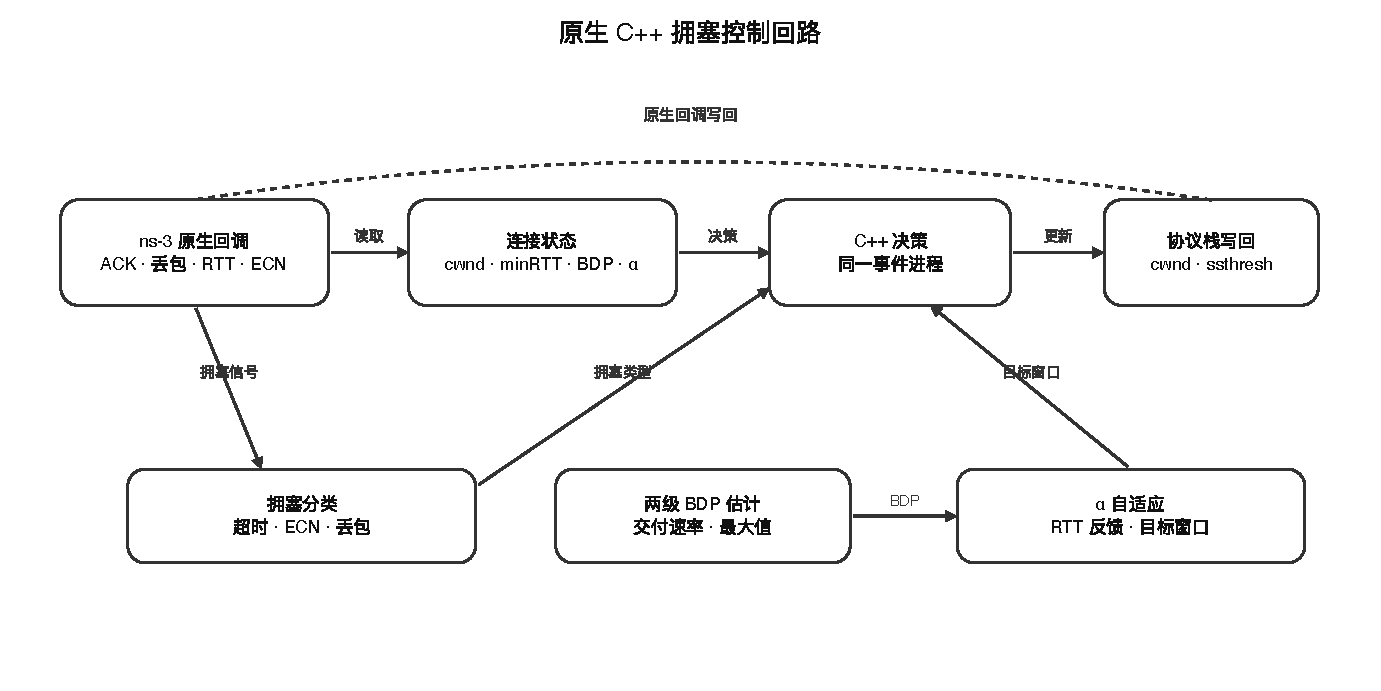
\includegraphics[width=0.86\textwidth]{plots/fig06_architecture_zh.pdf}
\caption{Swift控制回路总体架构：协议栈回调采集的状态向量经跨进程同步信道送入启发式决策模块，依次执行拥塞三分类判定、两级BDP估计与基线相对反馈自适应，ssthresh/cwnd决策经应答写回协议栈}
\label{fig:architecture}
\end{figure*}

Swift的决策问题可描述为一个\emph{事件驱动决策回路}：在\texttt{GetSsThresh}与\texttt{IncreaseWindow}回调上，以当前状态向量$s$（11维有效状态，嵌入于15元素传输容器，另含4项元数据通道）为输入，由确定性规则输出$\langle new\_ssThresh, new\_cWnd \rangle$。性能反馈值$r_t$由环境按确认进度与RTT/拥塞代价合成，仅用于参数层的慢速调整（见第\ref{subsubsec:alpha}节），不构成策略训练信号。

状态向量设计遵循以下原则：（1）\textbf{实现相关性}——覆盖当前规则使用或记录的ECN状态、CA状态、窗口、在途字节和RTT等协议栈信息；（2）\textbf{可观测性}——参数均由ns-3回调接口提供；（3）\textbf{有界处理}——观测维数和每流历史缓冲区均固定，便于控制单次规则计算与状态开销。

\subsection{11维观测空间设计}

Swift的状态向量采用“11维有效状态子空间 + 4项元数据通道”的15元素\texttt{uint64}传输布局，如表\ref{tab:observation}所示。连接标识（socketUuid、nodeId）用于多流识别和状态隔离，envType与simTime用于环境标识和投递速率计算；窗口状态（ssThresh、cWnd）、传输状态（segmentSize、segmentsAcked、bytesInFlight）、时延测量（lastRtt、minRtt）以及回调与拥塞控制状态（calledFunc、caState、caEvent、ecnState）构成其余字段。前4项是跨进程路由与时序元数据；后11项被传递给决策模块，其中当前规则直接读取除caEvent外的字段，caEvent作为协议栈事件记录保留。因此，本文所称“11维观测”是传输容器的有效状态子空间，而非声称每一字段均进入当前版本的每个决策分支。

\begin{table}[htbp]
\centering
\caption{Swift 11维有效观测子空间（对应15元素容器索引4$\sim$14）}
\label{tab:observation}
\small
\begin{tabular}{clp{3.2cm}}
\toprule
\textbf{索引} & \textbf{参数} & \textbf{说明} \\
\midrule
4  & ssThresh & 慢启动阈值(B) \\
5  & cwnd & 拥塞窗口(B) \\
6  & segSize & 段大小(B) \\
7  & segmentsAcked & 确认段数 \\
8  & bytesInFlight & 在途字节数 \\
9  & lastRtt & 最近RTT($\mu$s) \\
10 & minRtt & 最小RTT($\mu$s) \\
11 & calledFunc & 回调类型(0/1) \\
12 & caState & CA状态(0-4) \\
13 & caEvent & CA事件(0-7) \\
14 & ecnState & ECN状态(0-5) \\
\bottomrule
\end{tabular}
\end{table}

状态设计中的三个协议栈内部字段为caState、caEvent和ecnState。\textbf{caState}反映TCP拥塞控制状态机的当前状态：CA\_OPEN（0，正常传输）、CA\_DISORDER（1，收到重复确认）、CA\_CWR（2，响应ECN缩减窗口）、CA\_RECOVERY（3，快速恢复中）、CA\_LOSS（4，重传超时后的丢包状态）。\textbf{caEvent}记录TX\_START、CWND\_RESTART、COMPLETE\_CWR、LOSS、ECN\_NO\_CE、ECN\_IS\_CE以及延迟/非延迟ACK事件（枚举值0--7）。\textbf{ecnState}反映ECN协商和标记状态：ECN\_DISABLED（0）、ECN\_IDLE（1）、ECN\_CE\_RCVD（2）、ECN\_SENDING\_ECE（3）、ECN\_ECE\_RCVD（4）、ECN\_CWR\_SENT（5）。

这些字段使协议栈内部语义可随窗口、RTT与在途字节等状态一并传输。当前实现的三分类分支直接使用calledFunc、caState和ecnState；caEvent由\texttt{CwndEvent}更新并保留在观测中。整个Python决策路径不包含神经网络推理。

\subsection{多信号融合拥塞检测}

Swift将拥塞信号分为三类，采用两级优先级层次结构进行综合判断，并引入连续递减保护机制防止窗口过度收缩。

\textbf{第一优先级——窗口收缩回调检测}：当$calledFunc = 0$时（\texttt{GetSsThresh}回调），Python规则按实现顺序解释收缩原因：若$caState = \text{CA\_LOSS}$，归类为超时；否则，若$ecnState \in \{\text{ECN\_CE\_RCVD}, \text{ECN\_ECE\_RCVD}\}$或$caState = \text{CA\_CWR}$，归类为ECN；其余情况归类为普通丢包。该顺序是代码中的确定性分类规则，不依赖未经测量的信号似然比。

\textbf{第二优先级——ECN状态直接检测}：在\texttt{IncreaseWindow}路径上，当$ecnState \in \{\text{ECN\_CE\_RCVD}, \text{ECN\_ECE\_RCVD}\}$时，规则同样进入ECN响应。该分支要求瓶颈队列实际执行CE标记；若队列不标记CE，则不会观察到相应状态。第\ref{subsec:setup}节中的实验统一使用启用ECN标记的RED队列，并对四种协议对称开启ECN。

\textbf{连续递减保护机制}：Swift维护连续递减计数器$d$。拥塞响应使$d$自增；降窗后的冻结路径不清零该计数器，冻结结束后进入非拥塞窗口更新路径时再重置。当$d>D_{max}=3$时，规则保持当前窗口并仍设置4个ACK事件的冻结计数，从而限制连续信号导致的进一步乘性缩减。以普通丢包保留因子0.70为例，前三次响应后的比例为$0.70^3\approx34.3\%$；该数值仅说明代码的累积缩减幅度，不构成优于其他算法的理论证明。

完整的多信号融合拥塞检测算法如算法\ref{alg:detect}所示。

\begin{algorithm}[htbp]
\caption{Multi-Signal Fusion Congestion Detection}
\label{alg:detect}
\small
\begin{algorithmic}[1]
\REQUIRE Observation $obs$, consecutive decrease counter $d$
\ENSURE $(is\_congested, \; type)$
\STATE \textbf{// Level-1: window-reduction callback (GetSsThresh)}
\IF{$obs.calledFunc = 0$}
    \IF{$obs.caState = \text{CA\_LOSS}$}
        \RETURN $(True, \; \text{TIMEOUT})$
    \ELSIF{$obs.ecnState \in \{\text{CE\_RCVD}, \text{ECE\_RCVD}\}$ \textbf{or} $obs.caState = \text{CA\_CWR}$}
        \RETURN $(True, \; \text{ECN})$
    \ELSE
        \RETURN $(True, \; \text{LOSS})$
    \ENDIF
\ENDIF
\STATE \textbf{// Level-2: ECN state inspection}
\IF{$obs.ecnState \in \{\text{CE\_RCVD}, \text{ECE\_RCVD}\}$}
    \RETURN $(True, \; \text{ECN})$
\ENDIF
\RETURN $(False, \; \text{NONE})$
\end{algorithmic}
\end{algorithm}

\subsection{差异化拥塞响应机制}

NewReno、CUBIC等丢包型算法通常以固定的乘性缩减规则响应拥塞，不同算法的具体保留因子并不相同，但其标准响应不会按本文所用的超时、普通丢包与ECN三类语义分别选择参数。Swift在当前实现中采用如下差异化窗口保留因子：

\begin{equation}
\begin{aligned}
new\_cwnd &= \rho \cdot cwnd, \\
\rho &= \begin{cases}
0.70 & \text{丢包(LOSS)} \\
0.75 & \text{ECN标记} \\
0.50 & \text{超时(TIMEOUT)}
\end{cases}
\end{aligned}
\end{equation}

这组参数体现一种工程化的严重程度排序：RED的CE标记可在丢包前出现，因此采用0.75的相对温和收缩；普通丢包采用0.70；CA\_LOSS所表示的重传超时采用0.50并重新进入慢启动。上述数值是当前实现的手工预设，而非由似然估计或最优性证明得到；仓库也未保存分别关闭这些机制的消融实验，因此本文仅将其解释为实现设计。

慢启动阈值更新为$new\_ssthresh = \max(\rho \cdot \min(cwnd, BDP), \; new\_cwnd)$，窗口下限为$4 \times MSS$。该写法将阈值参考量限制在当前窗口与BDP估计的较小者，并确保阈值不低于新窗口；其效果需结合后续实验观察，而不被表述为一般性最优结论。

此外，当前实现在拥塞响应路径上还包含三项与信号不确定性直接相关的安全约束。（1）\textbf{降窗后冻结}：每次进入拥塞响应即将冻结计数器置为4个ACK事件，且该赋值先于连续递减下限判定执行，因此即使响应被$D_{max}$抑制，队列仍获得排空窗口。（2）\textbf{超时重入慢启动}：当拥塞类型为超时时，除施加$\rho=0.50$外还重置慢启动标志与慢启动阶段最小RTT采样，使控制律回到指数上探而非在错误的BDP估计附近继续微调。（3）\textbf{陈旧动作丢弃}：由于GetSsThresh回调接收的是常量协议栈状态，Python侧返回的$cwnd$需缓存至下一次IncreaseWindow才能生效；若在此期间协议栈进入CA\_LOSS（重传超时已重置窗口），环境侧将直接丢弃该缓存动作，避免陈旧决策覆盖协议栈的丢包恢复过程。差异化响应算法如算法\ref{alg:response}所示。

\begin{algorithm}[htbp]
\caption{Differentiated Congestion Response}
\label{alg:response}
\small
\begin{algorithmic}[1]
\REQUIRE Current $cwnd$, congestion type $type$, consecutive decrease counter $d$, BDP estimate $bdp$
\ENSURE New window $new\_cwnd$, new threshold $new\_ssthresh$
\STATE $d \leftarrow d + 1$; \; consecutive increases $\leftarrow 0$
\STATE $freeze \leftarrow 4$ \COMMENT{Post-decrease freeze, armed before the floor test}
\IF{$d > D_{max}$}
    \STATE $new\_cwnd \leftarrow \max(cwnd, \; 4 \times MSS)$ \COMMENT{Freeze window}
    \STATE $new\_ssthresh \leftarrow new\_cwnd$
    \RETURN $(new\_cwnd, \; new\_ssthresh)$
\ENDIF
\IF{$type = \text{LOSS}$}
    \STATE $\rho \leftarrow 0.70$
\ELSIF{$type = \text{ECN}$}
    \STATE $\rho \leftarrow 0.75$
\ELSIF{$type = \text{TIMEOUT}$}
    \STATE $\rho \leftarrow 0.50$; \; re-enter slow start
\ENDIF
\STATE $new\_cwnd \leftarrow \max(\rho \times cwnd, \; 4 \times MSS)$
\STATE $new\_ssthresh \leftarrow \max(\rho \times \min(cwnd, \; bdp), \; new\_cwnd)$
\RETURN $(new\_cwnd, \; new\_ssthresh)$
\end{algorithmic}
\end{algorithm}

\subsection{启发式反馈自适应的参数调优}
\label{subsubsec:alpha}

Swift根据多种网络状态因素动态调整乘性增加因子$\alpha \in [0.85, 1.30]$（初始值1.10），控制拥塞避免阶段窗口增长速度。当前实现的调优逻辑基于RTT膨胀、反馈值EMA和连续增长趋势三个启发式维度。与固定阈值不同，RTT膨胀阈值随最小RTT增大而放宽，其设计意图是降低长RTT路径在BDP填充阶段过早收缩的可能性。

\textbf{基于最小RTT感知阈值的调整}：设$r = lastRtt/minRtt$。Swift首先根据$minRtt$计算松弛量$slack = 0.3 + 0.15\sqrt{\max(0,minRtt_{ms}-1)}$，并构造$low=1+slack$、$mid=1+2slack$、$high=1+4slack$三个动态阈值。当$r < low$时，说明队列驻留较低，$\alpha$按0.02或0.03小步增加；当$low \leq r < mid$时，$\alpha$仅增加0.01以维持温和探测；当$r > high$时，说明排队膨胀明显，$\alpha$按0.02或0.03收缩并重置连续增长计数器。

\textbf{基于反馈值基线相对比较的调整}：同时维护性能反馈值$r_t$的快速指数移动平均$\bar{r}_t = (1 - \eta) \bar{r}_{t-1} + \eta r_t$（$\eta=0.15$）与慢速基线$b_t = (1 - \eta_b)b_{t-1} + \eta_b r_t$（$\eta_b=0.02$）。仅当$\bar{r} > b + m$时令$\alpha \mathrel{+}=0.01$，当$\bar{r} < b - 4m$时令$\alpha \mathrel{-}=0.01$，其中$m = \max(0.25, 0.1|b|)$。环境在\texttt{IncreaseWindow}事件上定义$r = \min(0.5\,segmentsAcked, 5) - p_{rtt}$；仅当$lastRtt/RTT_{min}>1.5$时，$p_{rtt}=\min(0.3(lastRtt/RTT_{min}-1.5), 3)$。在\texttt{GetSsThresh}回调上，ECN、CA\_LOSS和其他丢包分别赋值$-3$、$-20$和$-10$。因此，调节条件主要比较快速EMA与慢速基线的相对偏移，同时动态裕量仍随基线绝对值变化。

\textbf{基于连续增长趋势的调整}：窗口连续增长超过8次时，规则令$\alpha \mathrel{+}=0.01$。所有调整均限制在$[0.85,1.30]$内，以约束无线、蜂窝和广域网参数剖面下的调整幅度；该边界是预设安全范围，而非经消融证明的最优区间。完整的$\alpha$自适应过程如算法\ref{alg:adapt}所示。

\begin{algorithm}[htbp]
\caption{RTT- and Reward-Aware Adaptive Parameter Tuning}
\label{alg:adapt}
\small
\begin{algorithmic}[1]
\REQUIRE Current $\alpha$, observation $obs$, consecutive increase count $g$, reward EMA $\bar{r}$, reward baseline $b$
\ENSURE Updated $\alpha$
\STATE $r \leftarrow obs.lastRtt \;/\; obs.minRtt$
\STATE $slack \leftarrow 0.3 + 0.15\sqrt{\max(0, obs.minRtt_{ms}-1)}$
\STATE $low \leftarrow 1+slack$; $mid \leftarrow 1+2slack$; $high \leftarrow 1+4slack$
\IF{$r < low$}
    \STATE $\alpha \leftarrow \alpha + (obs.minRtt_{ms}>5 ? 0.02 : 0.03)$; $g \leftarrow g+1$
\ELSIF{$r < mid$}
    \STATE $\alpha \leftarrow \alpha + 0.01$
\ELSIF{$r > high$}
    \STATE $\alpha \leftarrow \alpha - (obs.minRtt_{ms}>5 ? 0.03 : 0.02)$; $g \leftarrow 0$
\ENDIF
\STATE $m \leftarrow \max(0.25, \; 0.1\,|b|)$
\IF{$\bar{r} > b + m$}
    \STATE $\alpha \leftarrow \alpha + 0.01$
\ELSIF{$\bar{r} < b - 4m$}
    \STATE $\alpha \leftarrow \alpha - 0.01$
\ENDIF
\IF{$g > 8$}
    \STATE $\alpha \leftarrow \alpha + 0.01$
\ENDIF
\STATE $\alpha \leftarrow \text{clamp}(\alpha, \; 0.85, \; 1.30)$
\end{algorithmic}
\end{algorithm}

\subsection{融合控制策略}

Swift将BDP估计、目标窗口渐进逼近和安全边界约束相结合。BDP估计采用窗口最大值滤波器（Windowed Max-Filter）：投递速率由滑动时间窗口内的累计确认字节数计算，$DR = \Delta bytes_{acked} / \Delta t$，时间窗口跨度取$\min(\max(2 \times RTT_{min}, 5\,\text{ms}), 1\,\text{s})$，使速率反映ACK时钟（即瓶颈排空速率）而非单个ACK的载荷（后者会按每RTT的ACK数量成倍低估带宽）；速率样本存入容量为$W_{bw}=40$的滑动窗口队列，取窗口内最大值$BW_{max}$作为瓶颈带宽估计；RTT采样窗口容量为$W_{rtt}=40$，并持续跟踪全局最小RTT。BDP计算为$BDP = BW_{max} \times RTT_{min}$；当BDP估计无效时回退至当前窗口值。BDP估计算法如算法\ref{alg:bdp}所示。

\begin{algorithm}[htbp]
\caption{Windowed Max-Filter BDP Estimation}
\label{alg:bdp}
\small
\begin{algorithmic}[1]
\REQUIRE Flow state $state$, observation $obs$
\ENSURE BDP estimate
\STATE $state.bytes_{acked} \leftarrow state.bytes_{acked} + obs.segAcked \times obs.segSize$
\STATE $W \leftarrow \min(\max(2 \times RTT_{min}, \; 5\,\text{ms}), \; 1\,\text{s})$ \COMMENT{Rate window span}
\STATE $dr \leftarrow \Delta bytes_{acked} \;/\; \Delta t$ over the last $W$ \COMMENT{Delivery rate}
\STATE $state.bw\_samples$.append($dr$) \COMMENT{Sliding window, capacity $W_{bw}=40$}
\STATE $BW_{max} \leftarrow \max(state.bw\_samples)$
\STATE $RTT_{min} \leftarrow \min(state.min\_rtt, \; obs.minRtt)$
\STATE $bdp \leftarrow BW_{max} \times RTT_{min}$
\IF{$bdp \leq 0$}
    \STATE $bdp \leftarrow \max(obs.cwnd, \; 1)$ \COMMENT{Fallback}
\ENDIF
\RETURN $bdp$
\end{algorithmic}
\end{algorithm}

\textbf{慢启动阶段}（$cwnd < ssthresh$）：目标窗口$target = 2 \times BDP$（下限$10 \times MSS$）。Swift采用HyStart风格退出规则：当当前RTT超过慢启动阶段最小RTT的动态阈值时结束慢启动；阈值按最小RTT分段取1.25、1.30或1.40，其设计意图是在短RTT路径上较早响应RTT膨胀，并在长RTT路径上保留更宽松的填充空间。标准增量为$segmentsAcked \times MSS$；仅当$cwnd<0.3BDP$且$lastRtt<1.2RTT_{min}$时，增量提升为$2 \times segmentsAcked \times MSS$。

\textbf{拥塞避免阶段}（$cwnd \geq ssthresh$）：当前实现先计算目标窗口$target=\alpha \times BDP$（BDP无效时回退到当前窗口），再以有界步长向目标靠拢。当$target>cwnd$时，窗口按$\max(\gamma\times MSS, MSS, (target-cwnd)/16)$上探，并以$target+\gamma\times MSS$为本次上限；该规则以当前差值的$1/16$作为候选步长，但不宣称固定在16个ACK事件内完成收敛。当$target<cwnd$时，每个ACK事件按$\max((cwnd-target)/2, MSS)$回落且不低于$target$；当二者相等时，按$\gamma\times MSS$执行每事件加性增长。当前实现取$\gamma=1.0$。若降窗冻结计数器非零，本次事件直接返回当前窗口并将计数器减一。

\textbf{管道利用率感知增量与安全边界}：管道利用率$u = bytesInFlight/cwnd$用于识别未充分填充的链路。该增量仅在$lastRtt < 1.3\,RTT_{min}$时生效：当$u<0.4$时，短RTT路径追加$2\times MSS$，最小RTT超过5 ms的长RTT路径追加$1\times MSS$；当$0.4 \leq u<0.5$时，仅短RTT路径追加$1\times MSS$。这一分级规则用于限制长RTT路径上的额外增量。最终窗口被约束在$[4\times MSS, \max(4\times BDP, 200\times MSS)]$内，以限制BDP估计陈旧时的窗口范围。融合控制策略的完整算法如算法\ref{alg:fusion}所示。

\begin{algorithm}[htbp]
\caption{Hybrid Rate-Window Fusion Control}
\label{alg:fusion}
\small
\begin{algorithmic}[1]
\REQUIRE Observation $obs$, parameter $\alpha$, BDP estimate $bdp$, freeze counter $f$
\ENSURE New window $new\_cwnd$
\IF{$f > 0$}
    \STATE $f \leftarrow f - 1$; \; \RETURN $obs.cwnd$ \COMMENT{Post-decrease freeze}
\ENDIF
\STATE $d \leftarrow 0$ \COMMENT{Reset after freeze on the non-congestion path}
\IF{$obs.cwnd < obs.ssthresh$ and flow is in slow start}
    \STATE Apply HyStart-style RTT-inflation exit ($1.25/1.30/1.40$ by $RTT_{min}$)
    \STATE $target \leftarrow \max(2 \times bdp, \; 10 \times MSS)$
    \STATE $\Delta \leftarrow obs.segmentsAcked \times MSS$
    \IF{$obs.cwnd < 0.3 \times bdp$ and $obs.lastRtt < 1.2\,RTT_{min}$}
        \STATE $\Delta \leftarrow 2 \times obs.segmentsAcked \times MSS$
    \ENDIF
    \STATE $new\_cwnd \leftarrow \min(obs.cwnd + \Delta, \; target)$
\ELSE
    \STATE $target \leftarrow \alpha \times bdp$
    \IF{$target > obs.cwnd$}
        \STATE $step \leftarrow \max(\gamma \times MSS, \; MSS, \; (target-obs.cwnd)/16)$
        \STATE $new\_cwnd \leftarrow \min(obs.cwnd + step, \; target + \gamma \times MSS)$
    \ELSIF{$target < obs.cwnd$}
        \STATE $new\_cwnd \leftarrow \max(obs.cwnd - \max(\tfrac{obs.cwnd-target}{2}, MSS), \; target)$
    \ELSE
        \STATE $new\_cwnd \leftarrow obs.cwnd + \gamma \times MSS$
    \ENDIF
\ENDIF
\IF{$obs.lastRtt < 1.3\,RTT_{min}$}
    \STATE $u \leftarrow obs.bytesInFlight / obs.cwnd$
    \IF{$u < 0.4$}
        \STATE $new\_cwnd \leftarrow new\_cwnd + (RTT_{min} > 5\,\text{ms} \; ? \; MSS : 2 \times MSS)$
    \ELSIF{$u < 0.5$ \textbf{and} $RTT_{min} \leq 5\,\text{ms}$}
        \STATE $new\_cwnd \leftarrow new\_cwnd + MSS$
    \ENDIF
\ENDIF
\STATE $new\_cwnd \leftarrow \text{clamp}(new\_cwnd, \; 4 \times MSS, \; \max(4 \times bdp, \; 200 \times MSS))$
\RETURN $new\_cwnd$
\end{algorithmic}
\end{algorithm}

\subsection{每流独立状态管理}

Swift为每个TCP连接维护独立状态，通过socketUuid为键的哈希表实现$O(1)$查找。每流状态包括四个子模块：（1）\textbf{带宽与RTT估计模块}——容量$W_{bw}=40$的投递速率滑动窗口队列和容量$W_{rtt}=40$的RTT采样队列，支持窗口最大值带宽估计、全局最小RTT追踪和慢启动阶段最小RTT采样；（2）\textbf{拥塞控制计数器}——连续递减计数器$d$、连续增长计数器$g$、累计丢包和ECN事件计数，以及降窗后的ACK冻结计数；（3）\textbf{性能指标聚合}——吞吐量指数移动平均、当前BDP估计、上一步窗口和时间戳；（4）\textbf{自适应参数}——$\alpha$（初始1.10）、$\gamma$（默认1.0）和慢启动标志位。

状态管理遵循延迟初始化（首次访问时创建）和增量更新（仅更新变化字段）两个原则。每流独立管理避免了多流并发场景下的流间干扰，支持差异化控制。反馈值EMA（平滑因子$\eta=0.15$）与慢速基线（$\eta_b=0.02$）由每个连接对应的决策实例独立维护，避免流间反馈串扰。

%========================================
% 4. 实验评估
%========================================

\section{实验评估}

\subsection{仿真配置与实验矩阵}
\label{subsec:setup}

\textbf{实现环境}：仿真基于ns-3.40\cite{ns3}与ns3-gym/OpenGym\cite{opengym}。Python进程执行Swift启发式控制，C++环境负责观测、动作应用、拓扑、业务和队列配置。现有实验记录不足以独立核验主机、操作系统与Python依赖版本，因此本文不报告这些版本，也不作运行时开销比较。

\textbf{拓扑与负载}：使用\texttt{PointToPointDumbbellHelper}构造哑铃拓扑，左右各3个叶子节点（$nLeaf=3$）经接入链路汇聚到一条共享瓶颈链路；每对叶子节点上运行一条\texttt{BulkSendHelper}长流，3条流分别在0.1、0.2与0.3 s启动，并统一在20.1 s停止，业务持续时间参数为20 s。MTU为1500 B，应用数据单元为1440 B，并启用SACK；瓶颈队列长度为$Q=\max(BDP \cdot nLeaf / MTU, \; 100)$个报文，其中$BDP$由瓶颈速率与完整基础RTT计算。

\textbf{队列管理与ECN}：瓶颈链路两端网关对称安装RED队列，标记下限$MinTh = 0.3Q$、上限$MaxTh = 0.9Q$、\texttt{UseEcn=true}，并对四种协议统一设置\texttt{TcpSocketBase::UseEcn=On}。

\textbf{A/B对照设置}：两组实验共享相同的场景参数、拓扑与随机运行号，每个配置执行一次确定性运行，仅\texttt{enable\_udp\_burst}取值不同：
\begin{itemize}
\item \textbf{纯TCP设置}：瓶颈上仅承载3条TCP长流；
\item \textbf{UDP突发设置}：在同一瓶颈上叠加一路OnOff UDP源。该源以1024 B报文按\texttt{On 0.5 s / Off 0.5 s}的50\%占空比运行，\emph{On期峰值速率取当前瓶颈速率的64\%}，长期平均负载为瓶颈速率的32\%。
\end{itemize}

\textbf{场景矩阵}：共36个场景，覆盖微秒级RTT近端高速链路、不同收敛比与拥塞程度的共享汇聚链路、非对称接入、WiFi命名配置、5G/LTE命名配置、城域/长途/跨域WAN以及LEO/GEO卫星链路；瓶颈速率10 Mbps$\sim$100 Gbps、基线RTT 4 $\mu$s$\sim$640 ms。每个场景在两种设置下各运行4种协议，合计$36\times4\times2=288$次仿真。场景名仅表示点到点链路的带宽与时延参数剖面；仿真未建立手机、笔记本或台式机硬件模型，也未使用真实WiFi、LTE、5G或卫星协议栈，因而只支持路径条件层面的结论。下文以19个代表性场景（S1--S19，表\ref{tab:scenarios}）展开，其余场景在第\ref{subsubsec:extended}节概述。

\textbf{对比算法与评测指标}：对比对象为NewReno\cite{newreno}、CUBIC\cite{cubic}与BBR\cite{bbr}。指标包括3条前向流的聚合有效吞吐量（Goodput，Mbps）、各前向流逐包平均单向端到端时延的非加权算术平均（ms）、按同样口径计算的抖动、汇总丢包率（\%）以及基于3条前向流吞吐量计算的Jain公平性指数\cite{fairness}。

\subsection{FlowMonitor测量口径}
\label{subsec:data-audit}

每条TCP连接在FlowMonitor中登记为前向数据流（10.1.x$\rightarrow$10.2.x，接收端口5000）与反向ACK流。为避免把ACK字节和ACK时延混入数据面指标，本文仅选择3条前向TCP数据流：吞吐量为3条前向流各自Goodput之和；场景时延与抖动先在每条流内按数据包求均值，再对3条流的均值作\emph{非加权算术平均}；丢包率由前向流丢包数与发送包数汇总计算；Jain指数由3条前向流的Goodput计算。

测量检查覆盖36场景、4协议和2设置形成的288次仿真。每次仿真均包含3条前向TCP流；指标满足吞吐量不超过瓶颈、时延不低于配置的基础单向时延以及Jain指数处于合法区间等约束。每个(场景, 协议, 设置)三元组只有一个随机运行号，本文不报告置信区间或统计显著性，并将结论限制在所考察的ns-3.40配置范围内。

表\ref{tab:scenarios}给出详细展开的19个代表性场景配置。为便于组织讨论，按路径特征将19个场景归为四组：\textbf{G1}为微秒级RTT近端高速链路，\textbf{G2}为近端共享/城域与跨域链路（100 Mbps$\sim$1 Gbps，含浅缓冲与深缓冲两类），\textbf{G3}为无线与蜂窝接入链路，\textbf{G4}为GEO卫星链路。

\begin{table}[htbp]
\centering
\caption{代表性19个场景配置（其余17个补充场景见正文第\ref{subsubsec:extended}节）}
\label{tab:scenarios}
\footnotesize
\setlength{\tabcolsep}{3.5pt}
\begin{tabular}{@{}ccllr@{}}
\toprule
\textbf{编号} & \textbf{组} & \textbf{场景} & \textbf{瓶颈(Mbps)} & \textbf{基础单向时延(ms)} \\
\midrule
S1 & G1 & intra\_rack\_10g & 10000 & 0.004 \\
S2 & G1 & intra\_rack\_25g & 25000 & 0.004 \\
S3 & G1 & leaf\_spine\_20g & 20000 & 0.009 \\
\midrule
S4 & G2 & asymmetric\_high & 1000 & 0.012 \\
S5 & G2 & congested\_heavy & 500 & 0.009 \\
S6 & G2 & symmetric\_low & 1000 & 0.030 \\
S7 & G2 & dc\_500m & 500 & 0.009 \\
S8 & G2 & dc\_100m & 100 & 0.009 \\
S9 & G2 & cross\_dc\_wan$^{\dagger}$ & 1000 & 5.020 \\
S10 & G2 & wan\_metro & 1000 & 2.200 \\
\midrule
S11 & G3 & wifi\_ac$^{\dagger}$ & 400 & 7.000 \\
S12 & G3 & wifi\_ax$^{\dagger}$ & 600 & 5.000 \\
S13 & G3 & wifi\_n & 50 & 14.0 \\
S14 & G3 & wifi\_legacy & 10 & 30.0 \\
S15 & G3 & nr\_5g\_embb$^{\dagger}$ & 500 & 7.000 \\
S16 & G3 & nr\_5g\_edge & 100 & 14.0 \\
S17 & G3 & lte\_good & 50 & 30.0 \\
S18 & G3 & lte\_poor & 10 & 70.0 \\
\midrule
S19 & G4 & satellite\_geo & 10 & 320.0 \\
\bottomrule
\end{tabular}
\vspace{2pt}

\raggedright
\scriptsize $\dagger$ 该场景未纳入图\ref{fig:udp-burst}和表\ref{tab:udp-burst-headline}详细展示的15个代表性配对子集（S1--S8、S10、S13、S14、S16--S19），但仍包含在36场景UDP突发聚合统计中。编号S1--S19为全文统一的场景标识。
\end{table}

\subsection{纯TCP设置下的传输性能}
\label{subsec:main-results}

表\ref{tab:throughput}、表\ref{tab:latency}与表\ref{tab:loss}分别给出19个代表性场景在纯TCP设置下的聚合吞吐量、前向流平均单向时延与丢包率（含Jain指数）。图\ref{fig:goodput-overview}与图\ref{fig:delay-overview}以对数坐标给出前两项指标（横轴为表\ref{tab:scenarios}中的场景编号）；黑色短划线标出配置的基础单向传播时延，柱体高出短划线的部分近似反映排队及其他仿真处理开销。

\begin{figure*}[!t]
\centering
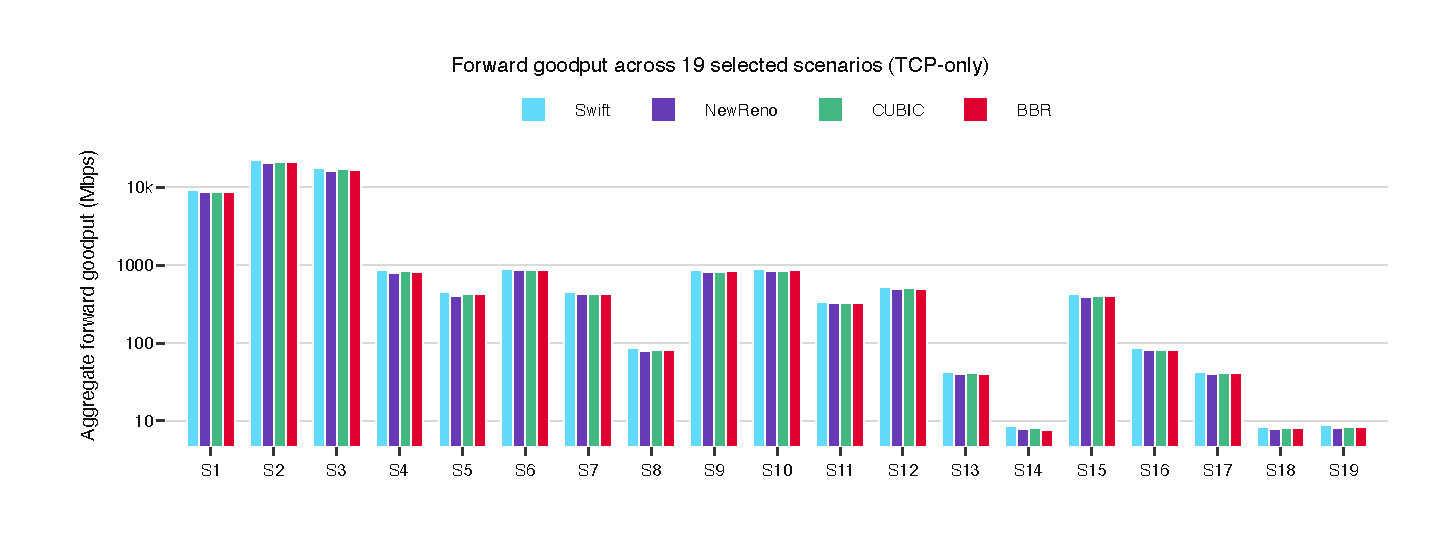
\includegraphics[width=0.92\textwidth]{plots/fig01_goodput_clean.pdf}
\caption{19个代表性场景的聚合前向吞吐量（对数坐标）。该子集中Swift整体呈现吞吐领先}
\label{fig:goodput-overview}
\end{figure*}

\begin{figure*}[!t]
\centering
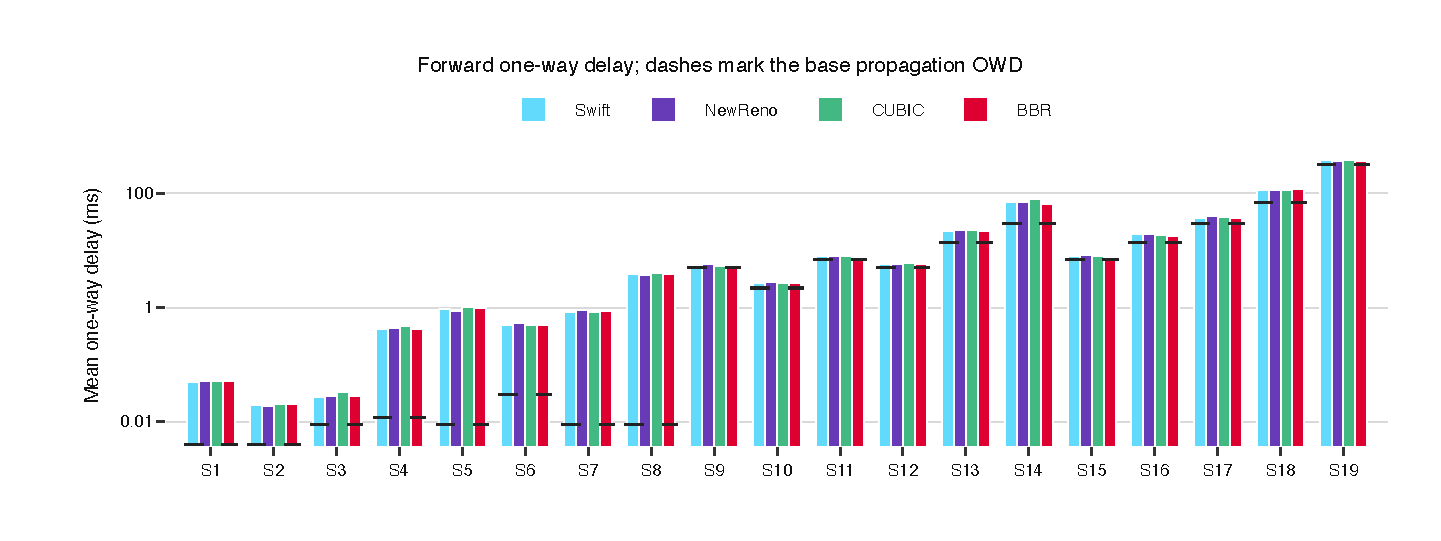
\includegraphics[width=0.92\textwidth]{plots/fig02_delay_clean.pdf}
\caption{19个场景的前向流平均单向时延（对数坐标；场景值为各流均值的非加权算术平均）。黑色短划线为基础单向传播时延}
\label{fig:delay-overview}
\end{figure*}

\begin{table}[htbp]
\centering
\caption{纯TCP设置：聚合有效吞吐量（Mbps，代表性19场景）}
\label{tab:throughput}
\scriptsize
\setlength{\tabcolsep}{3pt}
\begin{tabular}{@{}lrrrr@{}}
\toprule
\textbf{场景} & \textbf{Swift} & \textbf{NewReno} & \textbf{CUBIC} & \textbf{BBR} \\
\midrule
intra\_rack\_10g & 9302.6 & 8687.4 & 8865.0 & 8762.9 \\
intra\_rack\_25g & 22425.4 & 20483.8 & 21236.8 & 21161.4 \\
leaf\_spine\_20g & 18016.7 & 16279.4 & 17545.7 & 16805.3 \\
\midrule
asymmetric\_high & 878.6 & 798.6 & 839.7 & 817.0 \\
congested\_heavy & 454.5 & 406.8 & 430.3 & 429.6 \\
symmetric\_low & 905.0 & 886.5 & 886.5 & 886.5 \\
dc\_500m & 460.2 & 430.5 & 428.8 & 435.0 \\
dc\_100m & 86.7 & 80.1 & 82.2 & 81.1 \\
cross\_dc\_wan & 874.6 & 823.5 & 826.8 & 856.1 \\
wan\_metro & 909.4 & 844.4 & 860.4 & 863.4 \\
\midrule
wifi\_ac & 340.5 & 325.1 & 332.1 & 325.7 \\
wifi\_ax & 522.6 & 494.6 & 508.4 & 497.7 \\
wifi\_n & 42.7 & 40.0 & 41.3 & 40.8 \\
wifi\_legacy & 8.6 & 7.9 & 8.2 & 7.6 \\
nr\_5g\_embb & 429.5 & 399.0 & 408.6 & 402.2 \\
nr\_5g\_edge & 87.8 & 82.9 & 82.5 & 83.1 \\
lte\_good & 42.3 & 40.0 & 41.1 & 41.1 \\
lte\_poor & 8.5 & 7.9 & 8.1 & 8.2 \\
\midrule
satellite\_geo & 8.8 & 8.2 & 8.4 & 8.3 \\
\bottomrule
\end{tabular}
\end{table}

\begin{table}[htbp]
\centering
\caption{纯TCP设置：前向流均值的非加权平均单向时延（ms，代表性19场景）}
\label{tab:latency}
\scriptsize
\setlength{\tabcolsep}{3pt}
\begin{tabular}{@{}lrrrr@{}}
\toprule
\textbf{场景} & \textbf{Swift} & \textbf{NewReno} & \textbf{CUBIC} & \textbf{BBR} \\
\midrule
intra\_rack\_10g & 0.0502 & 0.0515 & 0.0524 & 0.0513 \\
intra\_rack\_25g & 0.0199 & 0.0190 & 0.0207 & 0.0206 \\
leaf\_spine\_20g & 0.0274 & 0.0279 & 0.0331 & 0.0281 \\
\midrule
asymmetric\_high & 0.4194 & 0.4292 & 0.4682 & 0.4203 \\
congested\_heavy & 0.9561 & 0.8742 & 1.0058 & 0.9892 \\
symmetric\_low & 0.5031 & 0.5385 & 0.5029 & 0.4958 \\
dc\_500m & 0.8489 & 0.9003 & 0.8516 & 0.8815 \\
dc\_100m & 3.9000 & 3.7952 & 4.0837 & 3.8845 \\
cross\_dc\_wan & 5.4327 & 5.7355 & 5.4350 & 5.2814 \\
wan\_metro & 2.6549 & 2.7965 & 2.7151 & 2.6598 \\
\midrule
wifi\_ac & 8.0957 & 8.1044 & 8.0509 & 7.7681 \\
wifi\_ax & 5.8703 & 5.8100 & 5.9325 & 5.7430 \\
wifi\_n & 22.2665 & 23.0975 & 23.2653 & 21.9797 \\
wifi\_legacy & 71.2199 & 72.2514 & 79.9873 & 64.5116 \\
nr\_5g\_embb & 8.0926 & 8.2075 & 7.9536 & 7.7523 \\
nr\_5g\_edge & 19.3383 & 19.2767 & 19.0235 & 18.2525 \\
lte\_good & 37.6320 & 39.5563 & 39.1253 & 37.4833 \\
lte\_poor & 114.4919 & 116.4265 & 115.4021 & 118.1664 \\
\midrule
satellite\_geo & 381.2900 & 378.8589 & 378.9036 & 367.2213 \\
\bottomrule
\end{tabular}
\end{table}

\begin{table*}[htbp]
\centering
\caption{纯TCP设置：丢包率（\%）与Jain公平性指数（代表性19场景）}
\label{tab:loss}
\scriptsize
\setlength{\tabcolsep}{2.5pt}
\begin{tabular}{@{}lrrrr|rrrr@{}}
\toprule
& \multicolumn{4}{c}{\textbf{丢包率 (\%)}} & \multicolumn{4}{c}{\textbf{Jain指数}} \\
\textbf{场景} & Swift & NewReno & CUBIC & BBR & Swift & NewReno & CUBIC & BBR \\
\midrule
intra\_rack\_10g & 0.018 & 0.021 & 0.021 & 0.022 & 1.000 & 0.999 & 1.000 & 0.999 \\
intra\_rack\_25g & 0.010 & 0.008 & 0.011 & 0.015 & 0.998 & 0.999 & 0.999 & 0.999 \\
leaf\_spine\_20g & 0.010 & 0.010 & 0.018 & 0.011 & 1.000 & 0.998 & 1.000 & 0.998 \\
asymmetric\_high & 0.017 & 0.011 & 0.017 & 0.016 & 0.999 & 0.998 & 0.996 & 1.000 \\
congested\_heavy & 0.015 & 0.015 & 0.016 & 0.021 & 0.999 & 0.999 & 0.994 & 0.989 \\
symmetric\_low & 0.021 & 0.020 & 0.022 & 0.021 & 1.000 & 0.996 & 0.999 & 1.000 \\
dc\_500m & 0.015 & 0.016 & 0.015 & 0.015 & 0.999 & 0.999 & 1.000 & 1.000 \\
dc\_100m & 0.008 & 0.009 & 0.013 & 0.009 & 0.999 & 1.000 & 0.999 & 0.997 \\
cross\_dc\_wan & 0.015 & 0.011 & 0.015 & 0.019 & 1.000 & 0.995 & 0.996 & 1.000 \\
wan\_metro & 0.021 & 0.011 & 0.023 & 0.024 & 1.000 & 1.000 & 1.000 & 0.999 \\
wifi\_ac & 0.014 & 0.014 & 0.014 & 0.017 & 0.997 & 0.999 & 0.999 & 0.992 \\
wifi\_ax & 0.012 & 0.013 & 0.013 & 0.018 & 1.000 & 0.999 & 0.999 & 1.000 \\
wifi\_n & 0.013 & 0.009 & 0.013 & 0.013 & 0.999 & 0.996 & 0.997 & 1.000 \\
wifi\_legacy & 0.021 & 0.023 & 0.022 & 0.000 & 0.998 & 0.995 & 0.996 & 0.996 \\
nr\_5g\_embb & 0.012 & 0.012 & 0.017 & 0.013 & 1.000 & 0.995 & 1.000 & 0.990 \\
nr\_5g\_edge & 0.019 & 0.020 & 0.017 & 0.017 & 0.999 & 0.996 & 0.999 & 0.993 \\
lte\_good & 0.013 & 0.009 & 0.013 & 0.017 & 0.998 & 0.998 & 0.991 & 1.000 \\
lte\_poor & 0.021 & 0.022 & 0.022 & 0.022 & 0.999 & 0.993 & 0.987 & 0.998 \\
satellite\_geo & 0.020 & 0.022 & 0.021 & 0.022 & 0.997 & 0.999 & 0.990 & 0.999 \\
\bottomrule
\end{tabular}
\end{table*}

\textbf{吞吐量}：在RED/ECN对称配置下，Swift在所考察场景中整体呈现吞吐领先。以逐场景NewReno/CUBIC/BBR中的最强吞吐基线为参照，36场景增益范围为2.1\%$\sim$5.8\%，中位数与均值均约4.1\%。代表性结果包括：\texttt{wan\_longhaul}为881.24 Mbps，较CUBIC高4.35\%；\texttt{wan\_metro}为909.37 Mbps，较BBR高5.32\%；\texttt{satellite\_leo}为134.95 Mbps，较BBR高4.77\%；\texttt{lte\_poor}为8.50 Mbps，较BBR高3.91\%；\texttt{dc\_500m}为460.17 Mbps，较BBR高5.79\%。这些结果覆盖长距离、无线/蜂窝命名参数剖面和近端链路，但不外推为真实异构终端硬件上的性能结论。

\textbf{时延}：Swift的时延总体与基线处于相近量级，但并非普遍最低。按未舍入复算结果，Swift严格时延最低的场景为7个，在21/36个场景中与逐场景最低时延相差不超过2\%。\texttt{wan\_longhaul}中Swift为26.1603 ms，较BBR低0.9\%；\texttt{wan\_metro}、\texttt{lte\_poor}与\texttt{dc\_500m}也呈现近优或最低时延。相反，\texttt{wifi\_legacy}、\texttt{nr\_5g\_edge}和\texttt{satellite\_geo}相对最低时延基线分别高10.4\%、5.9\%和3.8\%。这些差异表明吞吐领先与时延表现之间仍存在场景依赖的权衡，不能由单种子结果作统一因果归因。

\textbf{丢包与公平性}：36场景范围内四协议纯TCP丢包率上限为0.026\%。Swift严格丢包率最低仅见于8个场景，因而丢包表现应描述为与基线大体可比，而非系统性最优。Jain指数均接近1；Swift严格Jain最优的场景为11个，并在32/36个场景中距逐场景最优值不超过0.002。表\ref{tab:agg}保留均值与最小值以展示量级，不据此作“最均衡”的绝对结论。

\begin{table}[htbp]
\centering
\caption{全矩阵（36场景）丢包率与公平性聚合统计}
\label{tab:agg}
\scriptsize
\setlength{\tabcolsep}{3pt}
\begin{tabular}{@{}llcccc@{}}
\toprule
\textbf{设置} & \textbf{协议} & \textbf{丢包均值} & \textbf{丢包最大} & \textbf{Jain均值} & \textbf{Jain最小} \\
\midrule
纯TCP & Swift    & 0.0150 & 0.0225 & 0.9989 & 0.9967 \\
$n=36$ & NewReno & 0.0137 & 0.0227 & 0.9980 & 0.9933 \\
      & CUBIC   & 0.0176 & 0.0237 & 0.9977 & 0.9871 \\
      & BBR     & 0.0159 & 0.0259 & 0.9981 & 0.9888 \\
\midrule
UDP突发 & Swift   & 0.0279 & 0.0435 & 0.9990 & 0.9940 \\
$n=36$ & NewReno & 0.0269 & 0.0352 & 0.9976 & 0.9925 \\
      & CUBIC   & 0.0315 & 0.0431 & 0.9977 & 0.9877 \\
      & BBR     & 0.0287 & 0.0420 & 0.9983 & 0.9871 \\
\bottomrule
\end{tabular}
\vspace{2pt}

\raggedright
\scriptsize 丢包率单位为\%；Jain指数接近1表示3条前向流的吞吐分配接近均衡。均值和最小值仅用于量级比较。
\end{table}

\subsubsection{分组解读}

\textit{G1——微秒级RTT近端高速链路（S1--S3）}：瓶颈10$\sim$25 Gbps、基础单向时延4$\sim$9 $\mu$s。该组中Swift相对最强基线的吞吐增益为2.7\%$\sim$5.6\%。四协议时延为0.019$\sim$0.052 ms，差异处于数十微秒量级；这些结果表明该参数组中的吞吐提升未伴随数量级时延变化，但缺少队列轨迹和消融实验，不能进一步作机制因果归因。

\textit{G2——近端共享/城域/跨域链路（S4--S10）}：瓶颈100 Mbps$\sim$1 Gbps、基础单向时延0.012$\sim$5.02 ms，包含按BDP定尺缓冲与触及100包下界的配置。该组整体呈现2.2\%$\sim$5.8\%的吞吐增益。\texttt{wan\_metro}中Swift吞吐较BBR高5.32\%，时延2.6549 ms亦接近最低值；\texttt{dc\_500m}吞吐较BBR高5.79\%，且时延为该场景最低。\texttt{dc\_100m}中Swift时延3.9000 ms，较NewReno的3.7952 ms略高，体现了场景依赖的权衡。

\textit{G3——无线与蜂窝接入参数剖面（S11--S18）}：这些名称仅表示点到点链路的带宽与时延配置。该组总体呈现约2.5\%$\sim$5.7\%的吞吐增益；\texttt{lte\_poor}中Swift吞吐较BBR高3.91\%，时延114.49 ms为该场景最低。混合结果出现在\texttt{wifi\_legacy}与\texttt{nr\_5g\_edge}，Swift相对各自最低时延分别高10.4\%和5.9\%。

\textit{G4——GEO卫星参数剖面（S19）}：基础单向时延320 ms、瓶颈10 Mbps。Swift为8.78 Mbps，相对最强吞吐基线CUBIC的8.43 Mbps高4.15\%；其时延381.29 ms则比最低的BBR 367.22 ms高3.8\%。该结果同时体现长RTT配置下的吞吐收益与时延代价。

\subsubsection{补充场景：远距离与超高速链路的全矩阵覆盖}
\label{subsubsec:extended}

除表\ref{tab:scenarios}的19个场景外，全矩阵还包含17个补充场景，覆盖LEO卫星、长途WAN、跨Pod、叶脊扩展、100G近端、RDMA类、不同过订阅比例、拥塞梯度和混合流量配置。补充集合总体延续约2\%$\sim$6\%的吞吐领先趋势。LEO卫星参数剖面纯TCP为134.95 Mbps，较BBR的128.80 Mbps高4.77\%，UDP突发下为93.58 Mbps，较CUBIC的88.86 Mbps高5.31\%；长途WAN纯TCP为881.24 Mbps，较CUBIC高4.35\%，且时延较BBR低0.9\%。超高速参数剖面也显示吞吐提升，但RDMA类50 Gbps场景在UDP突发下相对最低时延高9.4\%，因此不能仅以吞吐指标概括补充集合。

\subsection{UDP突发跨流量鲁棒性评估}
\label{subsec:udp-burst}

手机、笔记本、台式机及其他端点所连接的共享路径可能同时承载突发性非响应式流量。本节在严格A/B对照下评估四协议在“平均负载为瓶颈速率32\%、On期峰值64\%、占空比50\%”的UDP突发干扰下的表现（第\ref{subsec:setup}节），并与纯TCP设置形成36组场景配对；该负载模拟共享路径上的跨流量，不代表具体终端硬件行为。

以同一场景的纯TCP结果为基准，表\ref{tab:udp-burst-agg}给出四种协议在36组配对上的吞吐量保持率$T_{udp}/T_{tcp}$、时延膨胀$D_{udp}/D_{tcp}-1$与新增丢包率。图\ref{fig:udp-burst}按15个代表性配对场景展示吞吐量变化与新增丢包。

\begin{table}[htbp]
\centering
\caption{UDP突发跨流量鲁棒性聚合指标（配对场景，$n=36$）}
\label{tab:udp-burst-agg}
\scriptsize
\setlength{\tabcolsep}{3pt}
\begin{tabular}{@{}lrrrc@{}}
\toprule
\textbf{协议} & \textbf{保持率均值} & \textbf{保持率最小} & \textbf{时延膨胀均值} & \textbf{新增丢包均值} \\
\midrule
Swift    & 68.6\% & 62.4\% & +2.9\% & +0.013 pp \\
NewReno & 68.6\% & 62.8\% & +3.1\% & +0.013 pp \\
CUBIC   & \textbf{68.8\%} & \textbf{63.9\%} & \textbf{+2.2\%} & +0.014 pp \\
BBR     & 68.7\% & 62.1\% & +3.3\% & +0.013 pp \\
\bottomrule
\end{tabular}
\vspace{2pt}

\raggedright
\scriptsize 保持率与时延膨胀按逐场景配对后取均值/最小值；新增丢包=突发设置丢包率$-$纯TCP设置丢包率。
\end{table}

\textbf{吞吐量}：UDP突发使四种协议的聚合吞吐量平均保持在纯TCP结果的68.6\%$\sim$68.8\%，其中Swift均值为68.6\%，与基线可比。就突发设置中的绝对吞吐量而言，Swift在所考察场景中多数呈现领先；相对逐场景最强基线的增益范围为2.2\%$\sim$5.9\%，中位数3.6\%，均值3.7\%。这表明当前单种子矩阵中未观察到其相对吞吐优势被明显削弱，但不能据此声称在其他突发强度或随机种子下必然保持。表\ref{tab:udp-burst-headline}给出15个代表性配对场景的绝对吞吐量与时延。

\textbf{时延、丢包与公平性}：UDP突发下Swift严格时延最低的场景为10个，在19/36个场景中与最低时延相差不超过2\%；严格Jain最优的场景为17个，在35/36个场景中距最优值不超过0.002；严格丢包率最低仅见于10个场景。总体上，公平性和丢包与基线接近，而非统一占优。混合时延结果包括\texttt{congested\_medium}、\texttt{nr\_5g\_edge}和\texttt{rdma\_like\_50g}，Swift相对最低时延分别高12.2\%、7.9\%和9.4\%。

\begin{figure*}[!t]
\centering
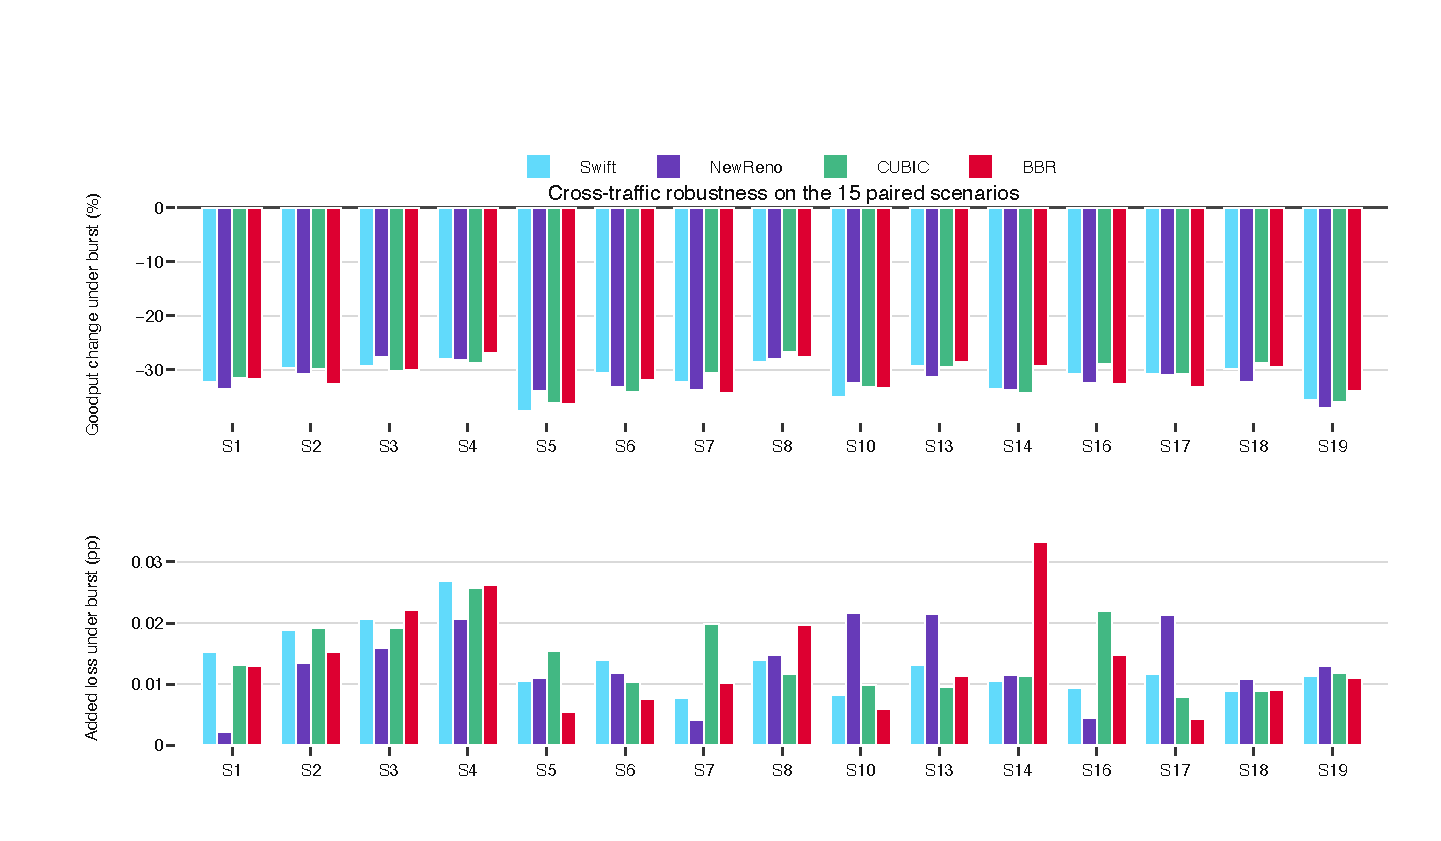
\includegraphics[width=0.92\textwidth]{plots/fig04_udp_burst_clean.pdf}
\caption{15个代表性配对场景的跨流量鲁棒性：UDP突发引起的吞吐量变化（上）与新增丢包（下，符号对数坐标）}
\label{fig:udp-burst}
\end{figure*}

\begin{table*}[htbp]
\centering
\caption{UDP突发设置下15个代表性场景的吞吐量与时延（吞吐量为前向流之和，时延为流均值的非加权平均）}
\label{tab:udp-burst-headline}
\footnotesize
\setlength{\tabcolsep}{4pt}
\begin{tabular}{@{}lrrrrrrrr@{}}
\toprule
\textbf{场景} & \multicolumn{4}{c}{\textbf{吞吐量 (Mbps)}} & \multicolumn{4}{c}{\textbf{平均单向延迟 (ms)}} \\
\cmidrule(lr){2-5} \cmidrule(lr){6-9}
 & Swift & NewReno & CUBIC & BBR & Swift & NewReno & CUBIC & BBR \\
\midrule
intra\_rack\_10g & 6295.2 & 5767.8 & 6063.1 & 5988.7 & 0.048 & 0.048 & 0.054 & 0.049 \\
intra\_rack\_25g & 15765.9 & 14181.8 & 14888.4 & 14268.4 & 0.020 & 0.020 & 0.023 & 0.020 \\
leaf\_spine\_20g & 12721.9 & 11782.0 & 12236.4 & 11754.9 & 0.030 & 0.031 & 0.034 & 0.030 \\
asymmetric\_high & 632.3 & 573.6 & 598.1 & 596.5 & 0.556 & 0.504 & 0.567 & 0.563 \\
congested\_heavy & 283.5 & 268.9 & 274.9 & 273.9 & 0.864 & 0.829 & 0.857 & 0.855 \\
symmetric\_low & 627.2 & 592.5 & 583.3 & 602.9 & 0.469 & 0.488 & 0.469 & 0.516 \\
dc\_500m & 311.8 & 285.3 & 297.2 & 285.4 & 0.908 & 0.890 & 0.957 & 0.862 \\
dc\_100m & 62.0 & 57.6 & 60.2 & 58.7 & 4.224 & 4.362 & 4.832 & 4.229 \\
wan\_metro & 591.2 & 570.6 & 574.7 & 575.7 & 2.609 & 2.747 & 2.625 & 2.693 \\
wifi\_n & 30.1 & 27.5 & 29.1 & 29.2 & 23.133 & 22.768 & 23.941 & 22.503 \\
wifi\_legacy & 5.7 & 5.2 & 5.4 & 5.4 & 73.369 & 73.677 & 75.589 & 74.655 \\
nr\_5g\_edge & 60.8 & 55.9 & 58.6 & 56.0 & 19.610 & 19.561 & 19.372 & 18.176 \\
lte\_good & 29.2 & 27.6 & 28.5 & 27.5 & 38.549 & 38.993 & 39.322 & 37.507 \\
lte\_poor & 6.0 & 5.4 & 5.7 & 5.8 & 117.590 & 111.634 & 123.046 & 122.328 \\
satellite\_geo & 5.7 & 5.1 & 5.4 & 5.5 & 361.464 & 381.743 & 354.523 & 363.152 \\
\bottomrule
\end{tabular}
\end{table*}

\textbf{远距离场景在突发下的表现}：GEO卫星参数剖面（S19）中Swift为5.65 Mbps，较最强吞吐基线BBR高3.29\%；LEO卫星参数剖面中Swift为93.58 Mbps，较CUBIC高5.31\%。\texttt{wan\_metro}在突发下为591.17 Mbps，较BBR高2.69\%，且时延接近该场景最低值。这些结果说明所测长RTT与城域参数剖面中仍观察到吞吐收益；由于没有机制消融、更多随机种子或真实链路实验，不能将该现象单独归因于某一控制模块。

\subsection{机制一致性与证据边界}

\textit{实现一致的解释}：Swift在ECN、普通丢包和超时路径上分别使用0.75、0.70和0.50的保留因子，并结合4个ACK事件冻结、滑动时间窗累计ACK投递速率、40样本最大值滤波以及$\alpha\times BDP$目标窗口跟踪。这些机制与“在RED/ECN环境下保留较充分的发送窗口，同时限制重复缩减和单ACK速率噪声”的解释相容。相比之下，NewReno、CUBIC与BBR具有不同的控制律。本文未测量逐协议在途窗口与队列轨迹，也未执行逐机制关闭的消融仿真，因此不能由聚合指标证明某一机制是吞吐差异的唯一原因，也不对基线内部状态作未测量的因果判断。

\textit{混合结果与外推边界}：（1）Swift严格丢包率最优的场景在纯TCP和UDP突发下分别为8个和10个，故丢包只能描述为整体可比；（2）纯TCP下\texttt{wifi\_legacy}、\texttt{nr\_5g\_edge}和\texttt{satellite\_geo}存在3.8\%$\sim$10.4\%的相对时延抬升，UDP突发下\texttt{congested\_medium}、\texttt{nr\_5g\_edge}和\texttt{rdma\_like\_50g}存在7.9\%$\sim$12.2\%的抬升；（3）Swift的吞吐保持率均值68.6\%与基线68.6\%$\sim$68.8\%相当。上述观察仅对应按瓶颈速率比例缩放的单种子UDP负载，不外推到其他突发强度、队列管理方式或真实异构终端。
%========================================
% 5. 讨论
%========================================

\section{讨论}
\label{sec:discussion}

\subsection{实现性质与定性分析}

\textbf{有界更新性质}：在拥塞避免阶段，窗口以$\max(\gamma MSS,MSS,(target-cwnd)/16)$向上调整，或以不超过当前超出量的规则向$\alpha\times BDP$回落；最终窗口再钳位到$[4MSS,\max(4BDP,200MSS)]$。检测到ECN、普通丢包或超时时，窗口分别按0.75、0.70和0.50的保留因子处理，连续缩减计数与4个ACK事件冻结限制重复响应。上述性质可由代码直接检查，但本文未给出Lyapunov收敛证明，也不声称目标窗口在任意网络条件下都是稳定平衡点。

\textbf{复杂度与计算开销}：当前实现采用确定性规则。带宽样本与RTT样本队列容量均为40，累计ACK时间窗队列容量为4096，其余状态为固定数量的计数器和标量；因此在这些固定上限下，单次决策和每流存储开销均有界。窗口最大值搜索及时间窗清理的实际代价取决于队列内样本数，本文不将其简化为未经实测的固定运行时。仓库未保存独立的决策时延、CPU利用率或内存压测日志，故不报告具体硬件上的性能开销。

\textbf{解释边界}：超时、普通丢包与ECN的优先级及保留因子表达了工程化的响应强度排序。本文没有估计这些信号的条件概率、似然比或最优控制输入，也没有形式化证明连续缩减保护的收敛性；相关机制仅按实现行为和聚合仿真结果作定性讨论。

\subsection{与相关工作的详细对比}

\begin{table*}[htbp]
\centering
\caption{Swift与主要相关算法的特性对比}
\label{tab:comparison}
\footnotesize
\setlength{\tabcolsep}{2.5pt}
\begin{tabular}{@{}lcccc@{}}
\toprule
\textbf{特性} & \textbf{Swift} & \textbf{Gemini} & \textbf{Aurora} & \textbf{DCTCP} \\
\midrule
有效状态维度 & 11 & 流级统计 & 10 & N/A \\
ECN状态利用 & 是 & 否 & 否 & 是 \\
CA状态利用 & 是 & 否 & 否 & 否 \\
决策机制 & 规则 & 规则 & DNN & 公式 \\
在线调整对象 & 参数 & 参数 & 策略 & 固定状态量 \\
自适应粒度 & 每流/每事件 & 流组/分钟级 & 每决策 & 每RTT \\
决策位置 & 栈外进程 & 内核数据面 & 栈外/栈内 & 内核 \\
策略训练 & 无 & 无（贝叶斯搜索参数） & 需要 & 无 \\
差异化响应 & 是 & 否 & 否 & 比例ECN响应 \\
生产部署证据 & 无 & 有 & 无 & 有 \\
\bottomrule
\end{tabular}
\end{table*}

\textbf{vs. Gemini\cite{gemini}}：两者均保留可解释的白盒控制逻辑，但参数适配方式、决策位置和时间尺度不同。Gemini的Fusion固定在内核数据面，Booster在带外以分钟级、流组粒度用贝叶斯优化搜索参数；Swift不执行学习或搜索，而是在协议栈外按每个窗口调整事件运行确定性启发式规则，并用RTT与基线相对反馈调节每流$\alpha$。Swift还能读取ECN与CA状态机，以代码中的优先级规则区分ECE/CWR相关收缩、普通丢包和超时；其代价是每事件一次跨进程同步往返，当前形态适用于研究与仿真平台，尚不具备Gemini已有的生产部署证据。

\textbf{vs. Aurora\cite{aurora}}：Swift采用11维有效状态子空间（Aurora常用10维观测），并引入ECN和CA状态参数。Swift采用基于规则的确定性决策而非深度神经网络，无需训练即可运行，决策路径可逐分支解释。Aurora的优势在于神经网络的表示能力，代价是训练数据收集、模型更新与推理开销；Swift则以可解释规则和协议栈内部信号换取工程可控性。本文不主张Swift在策略表示能力上优于Aurora。

\textbf{vs. DCTCP\cite{dctcp}}：Swift直接读取ECN协议栈状态进行离散分类，而DCTCP依据一个RTT内的标记比例更新拥塞估计并按$1-\alpha/2$缩窗。Swift同时使用丢包、ECN与CA状态，并设置0.70/0.75/0.50三类保留因子；其$D_{max}$与冻结计数是限制连续离散响应的工程机制。本文未在当前实验矩阵中纳入DCTCP，因而不作二者性能优劣结论。

\textbf{vs. BBR\cite{bbr}}：Swift综合ECN、CA状态与RTT等信号，并以$\alpha \times BDP$有界目标窗口调整cwnd；BBR则依赖瓶颈带宽、最小RTT估计和周期性增益循环。在所考察场景中，Swift相对逐场景最强吞吐基线的纯TCP增益为2.1\%$\sim$5.8\%，而UDP突发下Swift与BBR的吞吐保持率均值分别为68.6\%和68.7\%。时延结果更为混合：Swift在21/36个纯TCP场景中距最低值不超过2\%，但\texttt{wifi\_legacy}、\texttt{nr\_5g\_edge}和\texttt{satellite\_geo}相对最低时延仍高3.8\%$\sim$10.4\%。本文据此仅报告实现差异与观测结果，不推断未记录的内部机制因果关系。

\subsection{适用边界与未来方向}
\label{subsec:limitations}

\textit{在途窗口与时延的剩余代价}：Swift以$\alpha\times BDP$为目标且$\alpha$上界为1.30，部分配置中同时观察到吞吐提升与相对时延上升。纯TCP下\texttt{wifi\_legacy}、\texttt{nr\_5g\_edge}和\texttt{satellite\_geo}相对最低时延分别高10.4\%、5.9\%和3.8\%；UDP突发下\texttt{congested\_medium}、\texttt{nr\_5g\_edge}和\texttt{rdma\_like\_50g}分别高12.2\%、7.9\%和9.4\%。由于没有窗口/队列消融数据，本文不把这些差异唯一归因于$\alpha$。可探索的方向包括引入排队时延估计$q_{est}=RTT_{smoothed}-RTT_{min}$、在持续RTT膨胀时收紧$\alpha$，以及采用多时间尺度BDP估计。

\textit{参数预设依赖}：保留因子（0.70/0.75/0.50）、$\alpha$边界（$[0.85,1.30]$）、连续递减阈值（$D_{max}=3$）与降窗后冻结的ACK事件数（4）均为手动调优的预设值。未来可通过元学习\cite{meta_learning}或如Gemini\cite{gemini}所示的带外贝叶斯优化实现参数的在线搜索，二者可与本文的每事件决策回路组合成分层结构。

\textit{深度/学习型策略增强}：当前基于规则的启发式策略可解释性强但表示能力有限。后续若引入学习型组件（如离线强化学习训练、再经模型蒸馏提取规则），须在完整实验矩阵与异常过滤流程上重新评估，本文不将其作为当前系统的组成部分。

\textit{部署代价与真实环境验证}：每个窗口调整事件一次跨进程往返是当前实现的主要部署障碍。后续需将决策逻辑内联为Linux内核TCP模块或QUIC用户态拥塞控制插件，并在覆盖无线/蜂窝接入、广域网与卫星链路的真实或半实物测试床上验证。仿真与真实环境的差异（NIC offload、中断合并、NUMA效应、终端操作系统调度与无线链路波动）可能显著影响实际性能。

\textit{证据边界说明}：本文的测量来自36个链路参数剖面、4种协议和纯TCP/UDP突发两类设置下的ns-3.40 FlowMonitor前向流统计。每个配置只有一个随机运行号，不提供置信区间或显著性检验；场景采用RED/ECN对称配置并通过点到点链路参数抽象WiFi、蜂窝、WAN和卫星条件，不是异构终端硬件或真实接入协议验证。现有结果支持“在所考察场景中整体呈现约2\%$\sim$6\%吞吐领先、时延/丢包/公平性表现混合且总体可比”的表述，不支持普遍最优结论。

%========================================
% 6. 结论
%========================================

\section{结论}

本文提出了Swift——一种面向远距离传输、手机/笔记本/台式机等异构端点及多样接入与路径条件的启发式拥塞控制方法。其Python控制器经ns3-gym/OpenGym同步通道接收ns-3协议栈状态，并在\texttt{GetSsThresh}与\texttt{IncreaseWindow}事件上返回ssthresh/cwnd动作；该过程由确定性白盒规则完成，不依赖策略训练。核心技术贡献保持为三点：（1）\textbf{面向远距离与异构端点的多信号拥塞状态感知}，联合ECN、CA状态、RTT、最小RTT和在途字节等信息区分超时、ECN与普通丢包；（2）\textbf{ns3-gym集成的事件驱动启发式融合控制}，以滑动时间窗累计ACK投递速率和最小RTT估计BDP，通过RTT、基线相对反馈与增长趋势调节每流$\alpha$并有界跟踪目标窗口；（3）\textbf{面向不确定拥塞信号的稳定性与安全机制}，采用0.70/0.75/0.50差异化保留因子、至多3次连续缩减、4个ACK事件冻结、$4MSS$下界、$\max(4BDP,200MSS)$上界以及CA\_LOSS下的陈旧动作失效。

在ns-3.40平台上，本文以36个链路/路径参数剖面、4种协议和纯TCP/UDP突发两种设置形成288条记录。纯TCP下，Swift在所考察场景中整体呈现吞吐领先，相对逐场景最强基线的增益为2.1\%$\sim$5.8\%（中位数与均值均约4.1\%）；严格时延最低的场景为7个，21/36个场景与最低时延相差不超过2\%；严格Jain最优为11个，32/36个场景距最优值不超过0.002；严格丢包率最优仅为8个。UDP突发下吞吐增益为2.2\%$\sim$5.9\%（均值3.7\%），吞吐保持率均值68.6\%且与基线可比；严格最低时延、严格Jain最优和严格丢包率最低的场景分别为10、17和10个。\texttt{wan\_longhaul}、\texttt{wan\_metro}、\texttt{satellite\_leo}、\texttt{lte\_poor}和\texttt{dc\_500m}提供了吞吐或吞吐--时延均较有利的代表性结果。

证据边界同样明确：\texttt{wifi\_legacy}、\texttt{nr\_5g\_edge}、\texttt{satellite\_geo}以及UDP突发下的\texttt{congested\_medium}、\texttt{rdma\_like\_50g}等场景存在3.8\%$\sim$12.2\%的相对时延抬升，公平性和丢包总体接近基线而非统一最优。每配置仅有一个随机种子，未开展消融、置信区间或显著性检验；场景名仅代表点到点链路参数剖面，不构成异构终端硬件级验证。后续工作包括多种子重复实验、队列/窗口轨迹与机制消融、突发强度扫描、真实或半实物端点测试，以及将每事件规则内联到内核或用户态协议栈以降低跨进程开销。

\bibliographystyle{IEEEtran}
\bibliography{NJUPT_Professional_Thesis_draft1/reference/Ref_Article,NJUPT_Professional_Thesis_draft1/reference/Ref_Conference,NJUPT_Professional_Thesis_draft1/reference/Ref_Book}

\end{document}
